For this case, the drug-eluting stent is placed on top of 
the curved channel. It is modeled by 10 uniformly spaced 
semi-circles. As in the previous case, an channel obstruction of 
40\% was considered due to atherosclerosis and the domain was 
discretized using 11807 nodes and 26426 linear triangular elements. 

\par 
The \ref{velocity evolution real stent} shows the unsteady velocity 
profile in the middle of the channel ($x=5R$). 
As we can see, the maximum non-dimensional value of the velocity field 
reaches $u=2.65$ when the stent is placed, that is, we have an 
increase of $18$\% when compared to the artery with only 
atherosclerosis as in the previous case 
(see section \ref{canal real}).
However, this increase of the velocity may vary according to the 
coronary artery geometry for each patient.

\begin{figure}[H]
     \centering
     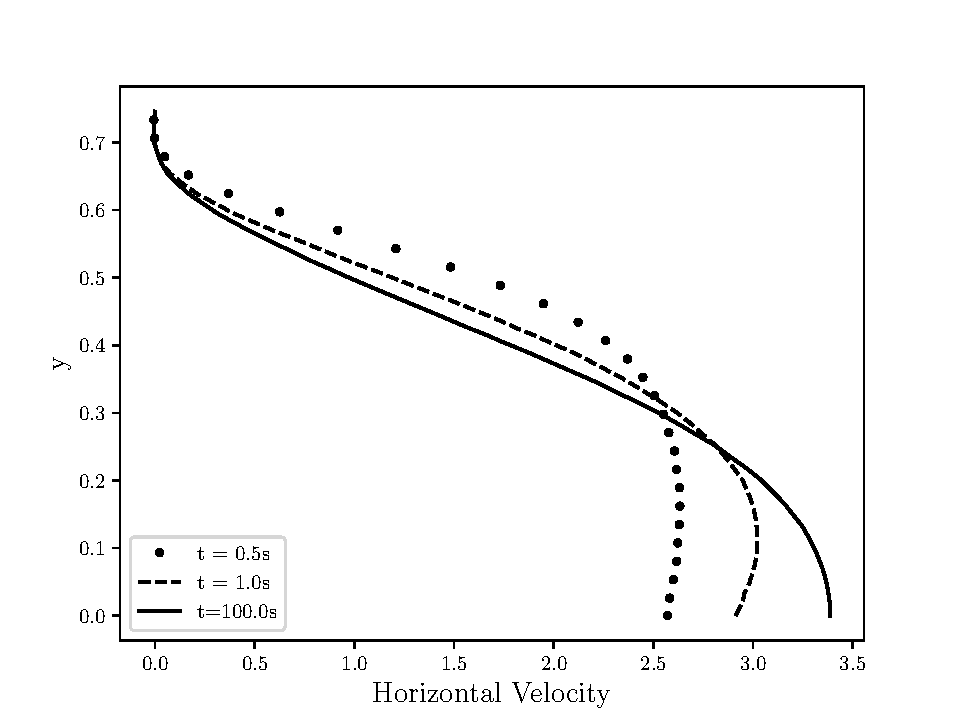
\includegraphics[scale=1]{./02_chaps/cap_solution/figure/vel_RealStrut_evol.pdf}\\
     \caption{
The unsteady velocity profile for real channel with drug-eluting stent.}
     \label{velocity evolution real stent}
\end{figure}

\newpage
The \ref{velocity field real stent} presents the evolution in 
time and space of the velocity field for half of the domain. 
The velocity field is represented with non-dimensional values 
where the red color refers to the $u=2.65$ value and the blue color 
$u=0$ value. Conveting to dimensional values, 
we have $u=31.8cm/s$ and $u=0cm/s$ respectively.

\vspace{2cm}
\begin{figure}[H]
     \begin{minipage}{.50\linewidth}
      \centering
      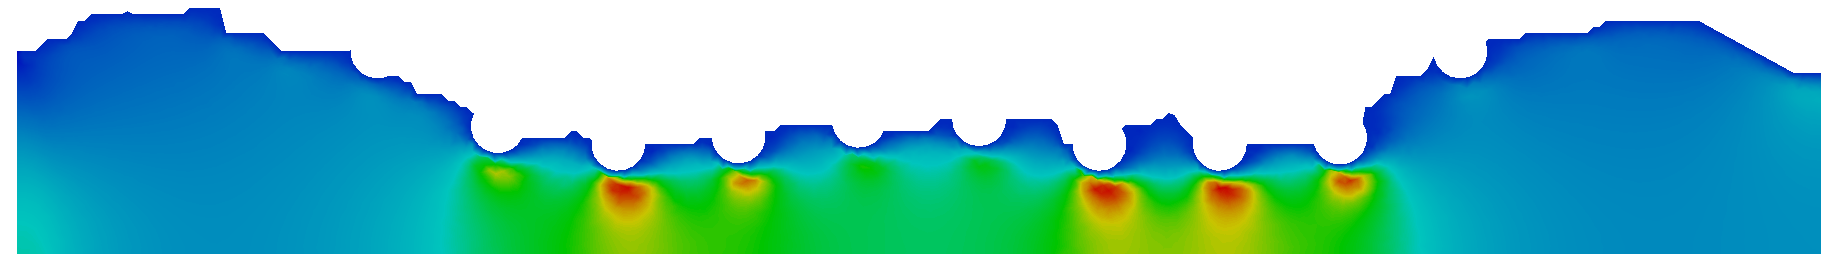
\includegraphics[scale=0.12]{./02_chaps/cap_solution/figure/vel_RealStrut200.png}\\
      t = 0.1
     \end{minipage}%
     \begin{minipage}{.50\linewidth}
      \centering
      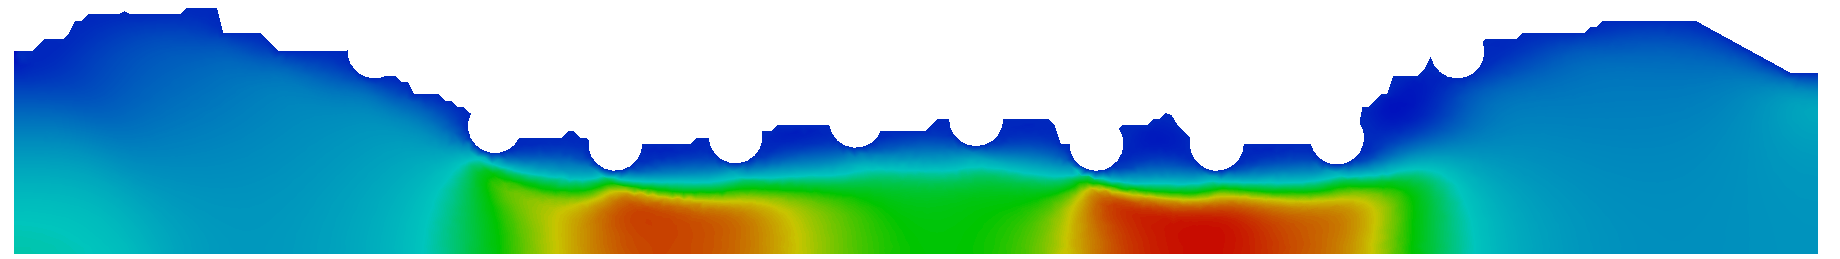
\includegraphics[scale=0.12]{./02_chaps/cap_solution/figure/vel_RealStrut1000.png}\\
      t = 0.5
     \end{minipage}
     \begin{minipage}{.50\linewidth}
     \medskip
      \centering
      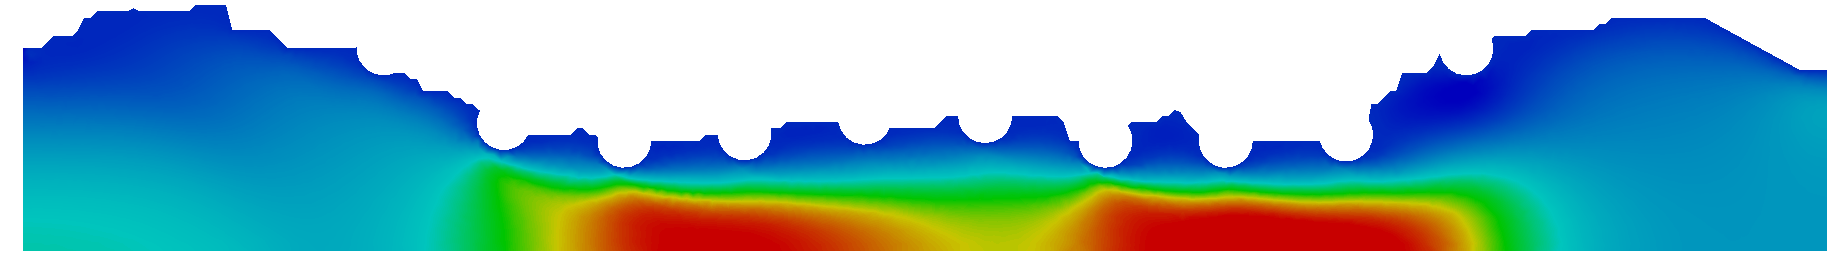
\includegraphics[scale=0.12]{./02_chaps/cap_solution/figure/vel_RealStrut2000.png}\\
      t = 1.0
     \end{minipage}%
     \begin{minipage}{.50\linewidth}
     \medskip
      \centering
      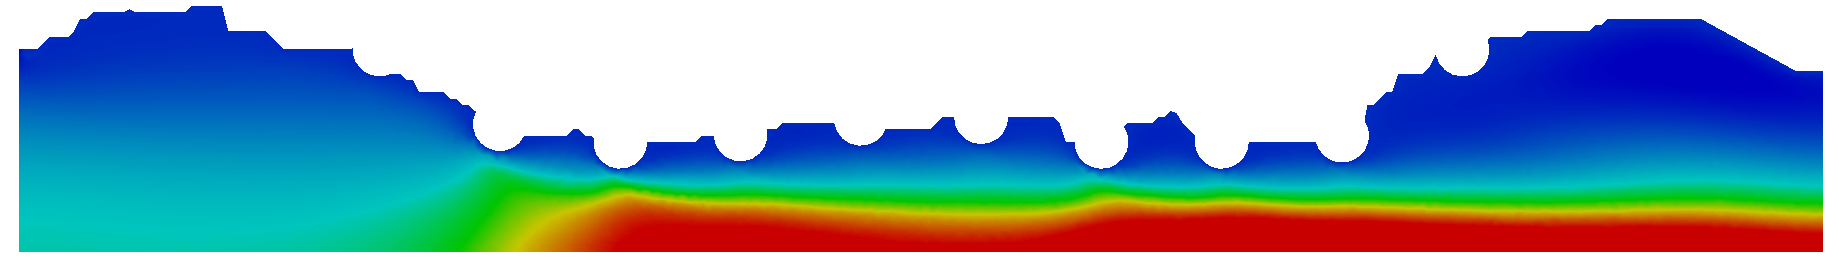
\includegraphics[scale=0.12]{./02_chaps/cap_solution/figure/vel_RealStrut6000.png}\\
      t = 3.0
     \end{minipage}
     \begin{minipage}{.50\linewidth}
      \centering
      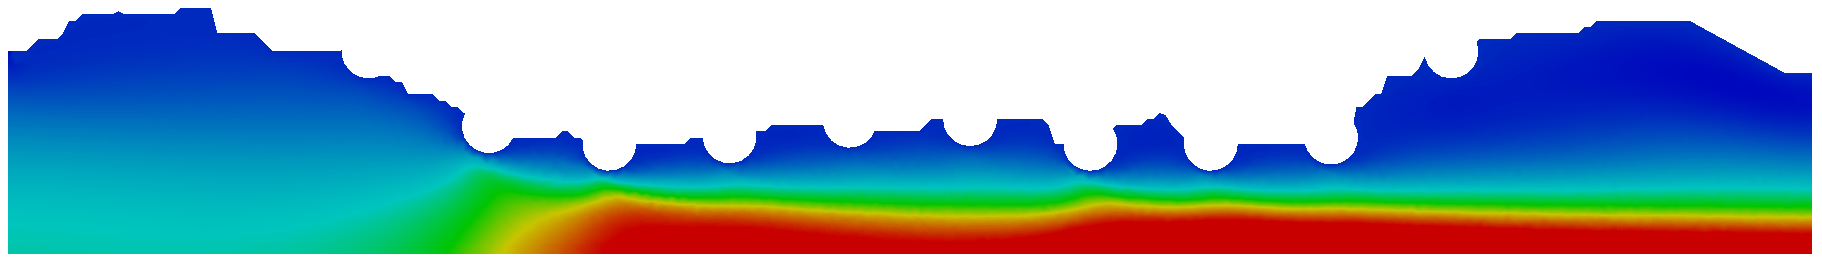
\includegraphics[scale=0.12]{./02_chaps/cap_solution/figure/vel_RealStrut8000.png}\\
      t = 4.0
     \end{minipage}%
     \begin{minipage}{.50\linewidth}
      \centering
      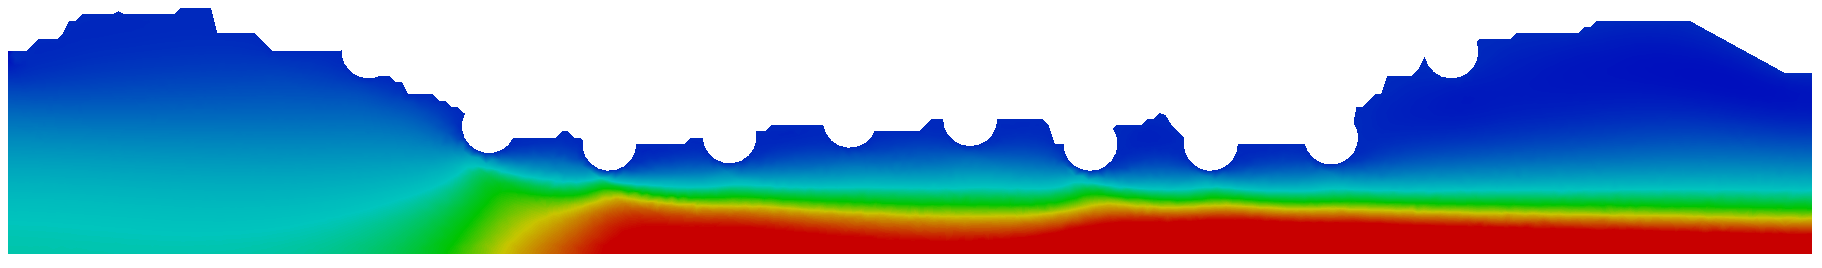
\includegraphics[scale=0.12]{./02_chaps/cap_solution/figure/vel_RealStrut10000.png}\\
      t = 5.0
     \end{minipage}
     \begin{minipage}{.50\linewidth}
     \medskip
      \centering
      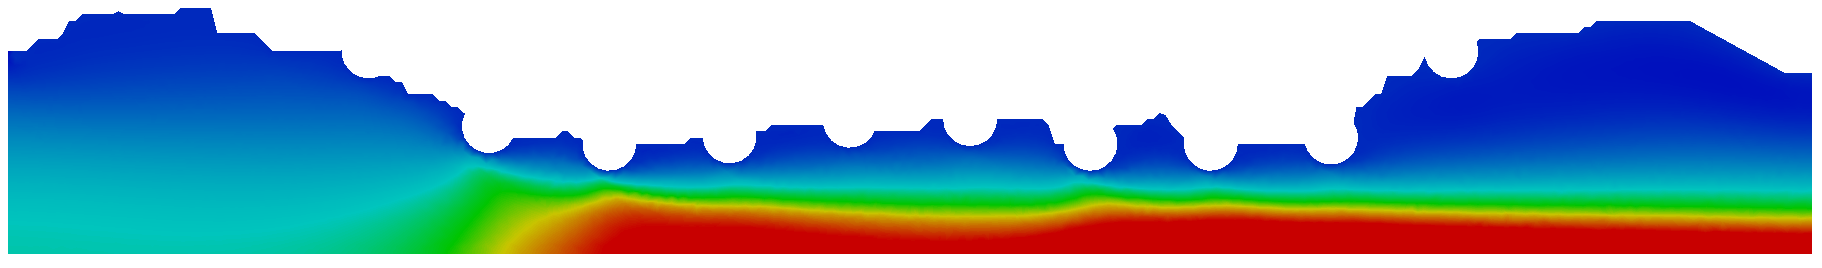
\includegraphics[scale=0.12]{./02_chaps/cap_solution/figure/vel_RealStrut14000.png}\\
      t = 7.0
     \end{minipage}%
     \begin{minipage}{.50\linewidth}
     \medskip
      \centering
      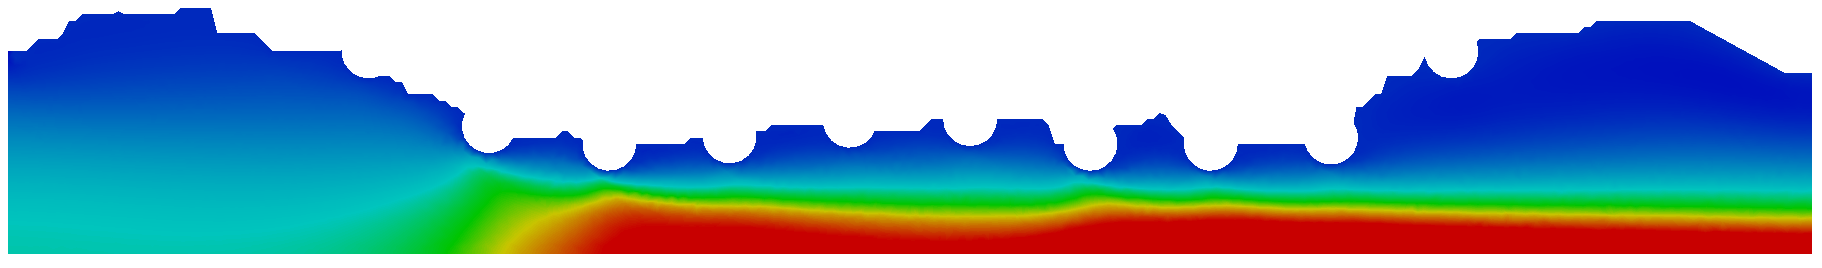
\includegraphics[scale=0.12]{./02_chaps/cap_solution/figure/vel_RealStrut20000.png}\\
      t = 10.0
     \end{minipage}
     \medskip
     \caption{
Time and space evolution of the velocity field for real channel with
drug-eluting stent.}
     \label{velocity field real stent}
\end{figure}

\vspace{1cm}
The \ref{conc field real stent sc 1} and 
\ref{conc field real stent sc 10} show the time and space evolution 
of the concentration field for several \textit{Schmidt} number, 
such as: $1$ and $10$ respectively. The concentration field is 
represented with the non-dimensional values where the red color 
represents $100$\% and the blue color represents $0$\% 
of the diffused concentration in the bloodstream. 
It is possible to observe that the \textit{Schmidt} number directly 
influences the drug transport in the blood flow. 
For high values of the \textit{Schmidt} number, 
the transport of chemical species becomes purely convective.

\begin{figure}[H]
     \begin{minipage}{.50\linewidth}
      \centering
      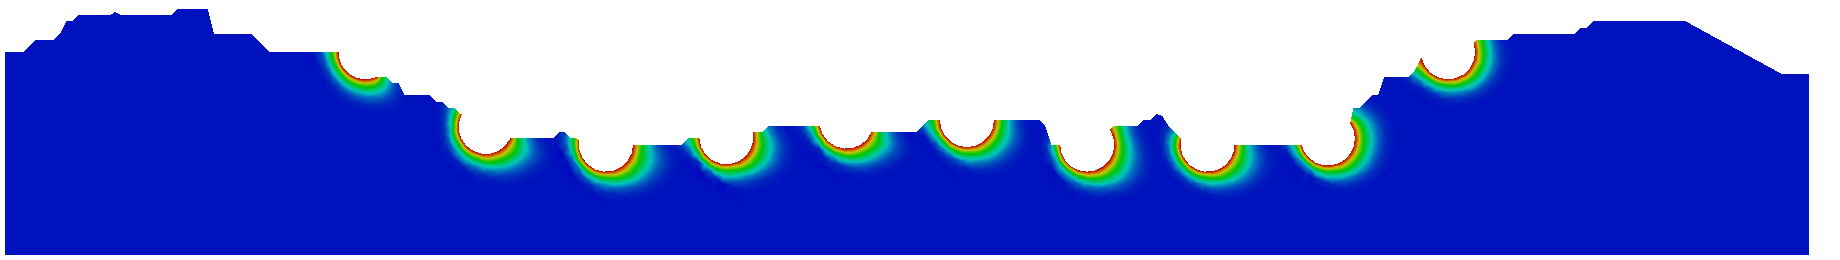
\includegraphics[scale=0.12]{./02_chaps/cap_solution/figure/conc1_RealStrut200.png}\\
      t = 0.1
     \end{minipage}%
     \begin{minipage}{.50\linewidth}
      \centering
      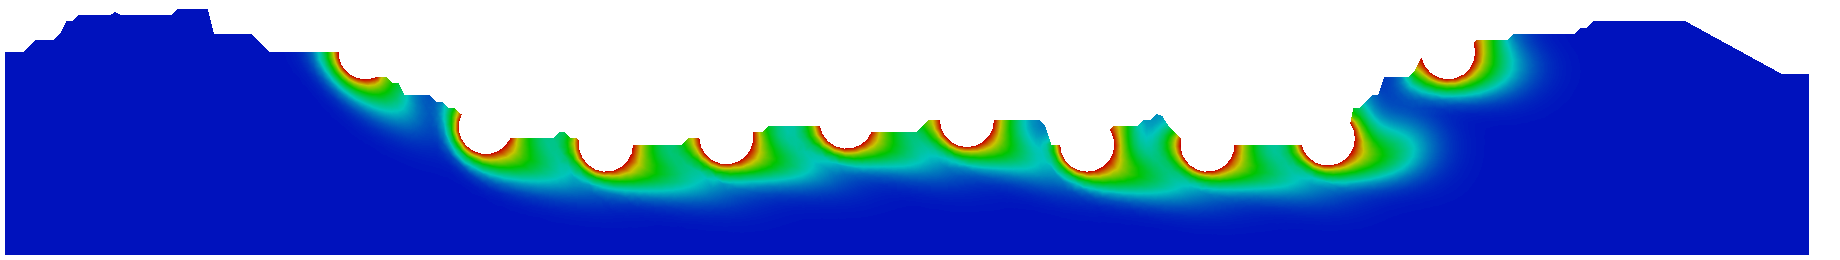
\includegraphics[scale=0.12]{./02_chaps/cap_solution/figure/conc1_RealStrut1000.png}\\
      t = 0.5
     \end{minipage}
     \begin{minipage}{.50\linewidth}
     \medskip
      \centering
      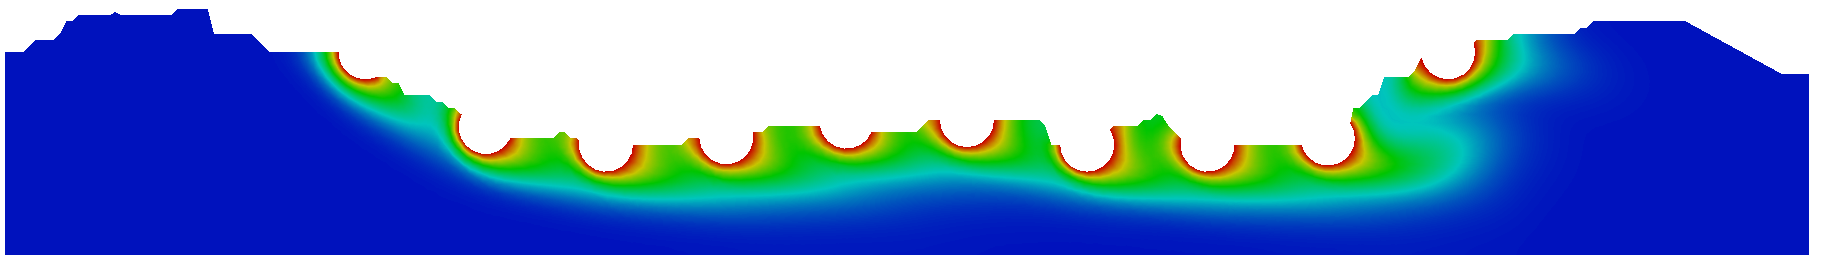
\includegraphics[scale=0.12]{./02_chaps/cap_solution/figure/conc1_RealStrut2000.png}\\
      t = 1.0
     \end{minipage}%
     \begin{minipage}{.50\linewidth}
     \medskip
      \centering
      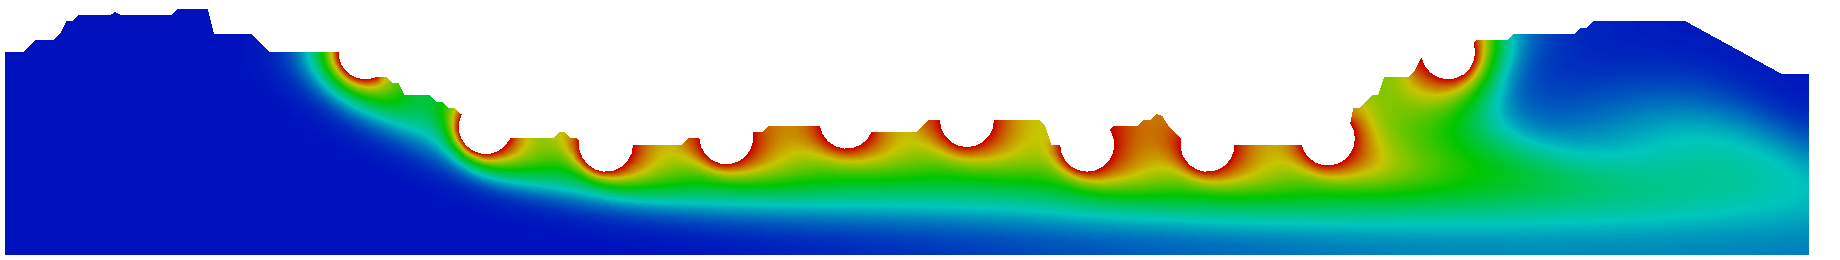
\includegraphics[scale=0.12]{./02_chaps/cap_solution/figure/conc1_RealStrut6000.png}\\
      t = 3.0
     \end{minipage}
     \begin{minipage}{.50\linewidth}
      \centering
      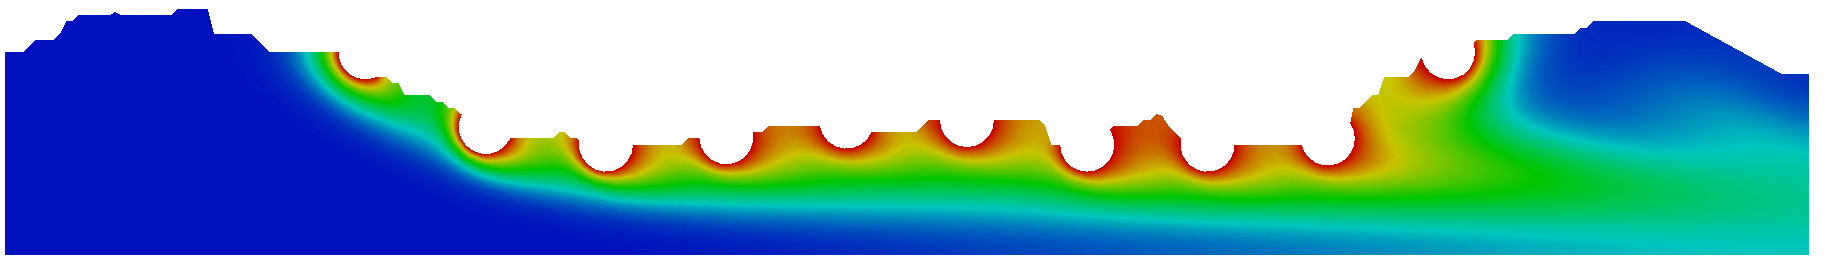
\includegraphics[scale=0.12]{./02_chaps/cap_solution/figure/conc1_RealStrut8000.png}\\
      t = 4.0
     \end{minipage}%
     \begin{minipage}{.50\linewidth}
      \centering
      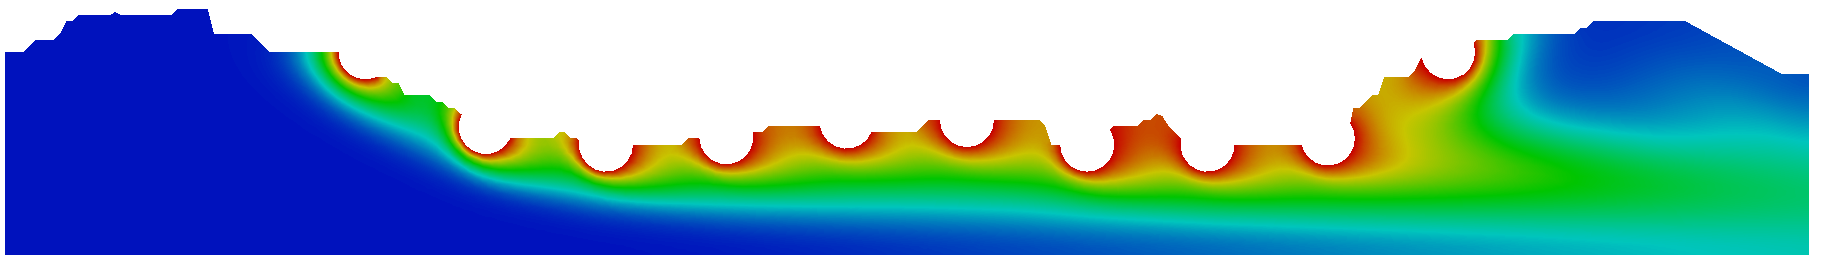
\includegraphics[scale=0.12]{./02_chaps/cap_solution/figure/conc1_RealStrut10000.png}\\
      t = 5.0
     \end{minipage}
     \begin{minipage}{.50\linewidth}
     \medskip
      \centering
      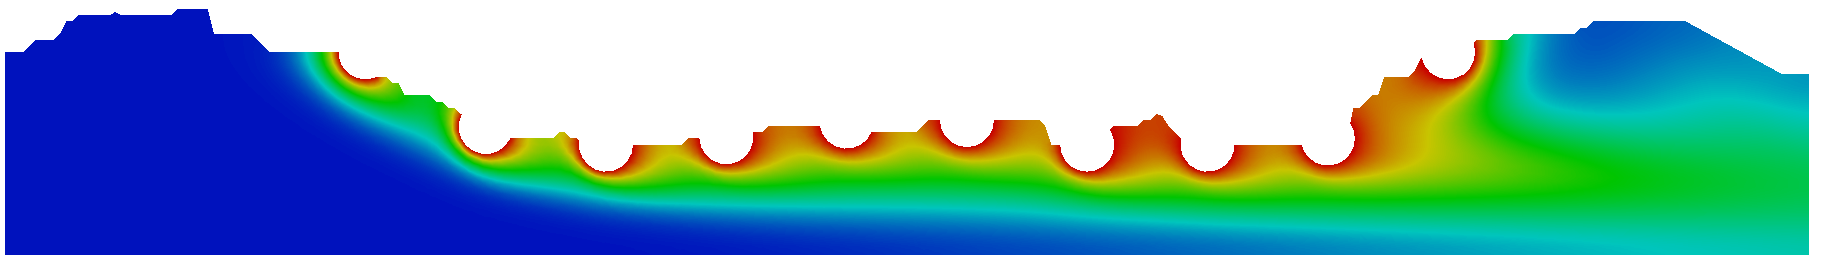
\includegraphics[scale=0.12]{./02_chaps/cap_solution/figure/conc1_RealStrut14000.png}\\
      t = 7.0
     \end{minipage}%
     \begin{minipage}{.50\linewidth}
     \medskip
      \centering
      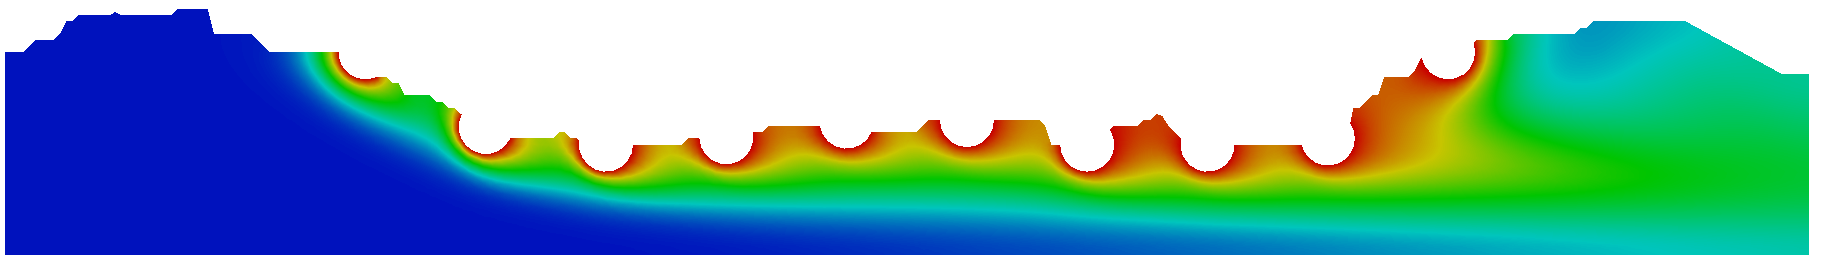
\includegraphics[scale=0.12]{./02_chaps/cap_solution/figure/conc1_RealStrut20000.png}\\
      t = 10.0
     \end{minipage}
     \medskip
     \caption{
Time and space evolution of the concentration field for real channel 
with drug-eluting stent when the $Sc=1$.}
     \label{conc field real stent sc 1}
\end{figure}

\bigskip
\begin{figure}[H]
     \begin{minipage}{.50\linewidth}
      \centering
      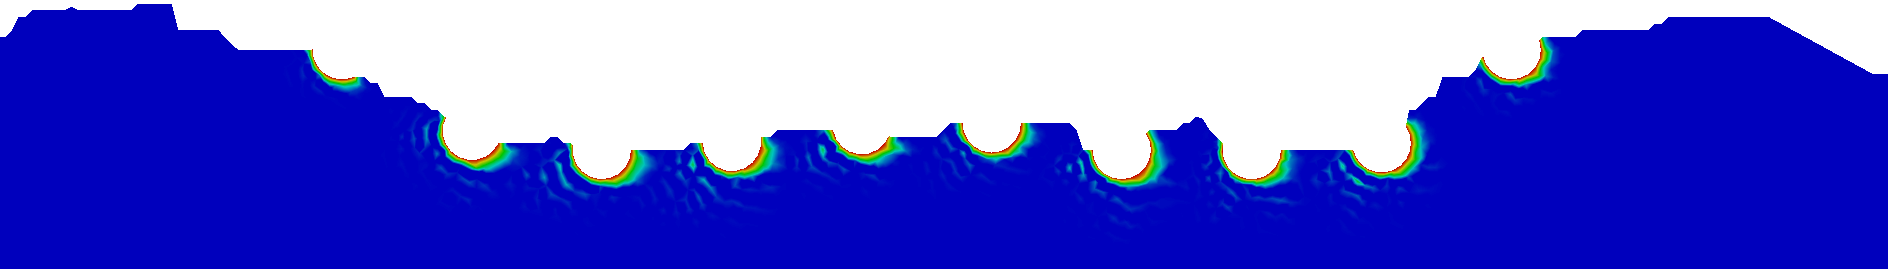
\includegraphics[scale=0.115]{./02_chaps/cap_solution/figure/conc10_RealStrut500.png}\\
      t = 0.1
     \end{minipage}%
     \begin{minipage}{.50\linewidth}
      \centering
      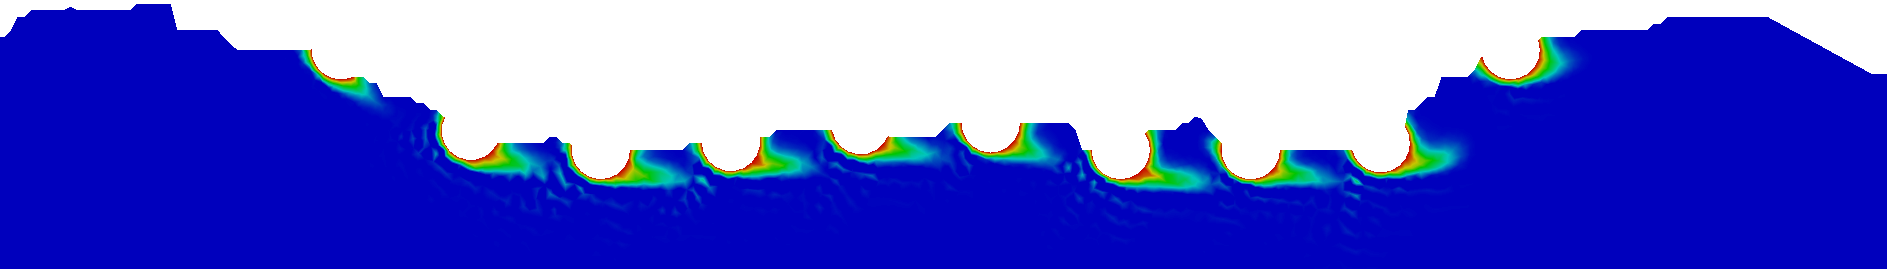
\includegraphics[scale=0.115]{./02_chaps/cap_solution/figure/conc10_RealStrut2500.png}\\
      t = 0.5
     \end{minipage}
     \begin{minipage}{.50\linewidth}
     \medskip
      \centering
      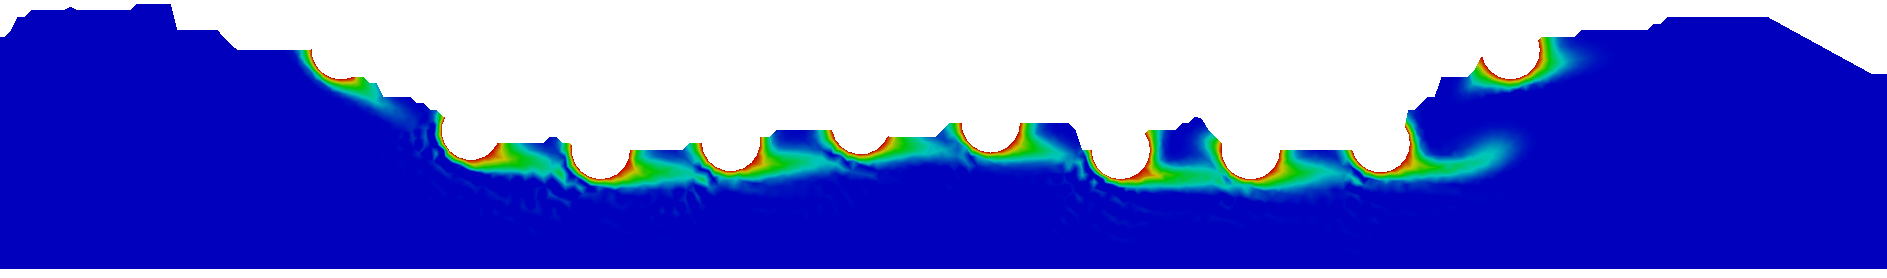
\includegraphics[scale=0.115]{./02_chaps/cap_solution/figure/conc10_RealStrut5000.png}\\
      t = 1.0
     \end{minipage}%
     \begin{minipage}{.50\linewidth}
     \medskip
      \centering
      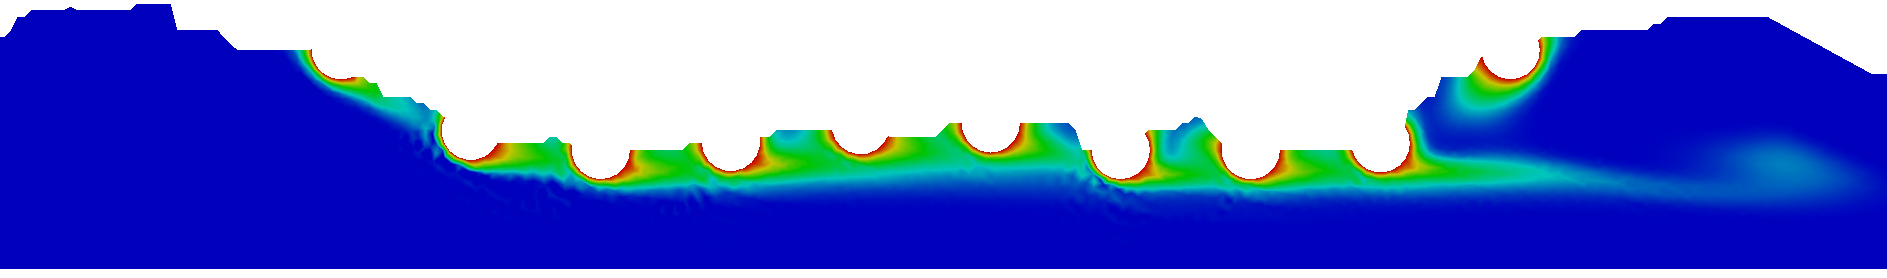
\includegraphics[scale=0.115]{./02_chaps/cap_solution/figure/conc10_RealStrut15000.png}\\
      t = 3.0
     \end{minipage}
     \begin{minipage}{.50\linewidth}
      \centering
      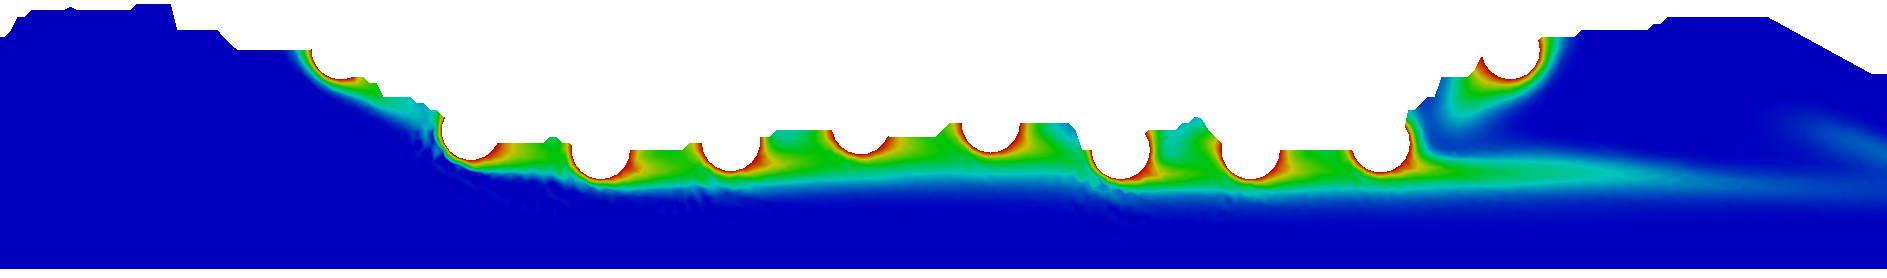
\includegraphics[scale=0.115]{./02_chaps/cap_solution/figure/conc10_RealStrut20000.png}\\
      t = 4.0
     \end{minipage}%
     \begin{minipage}{.50\linewidth}
      \centering
      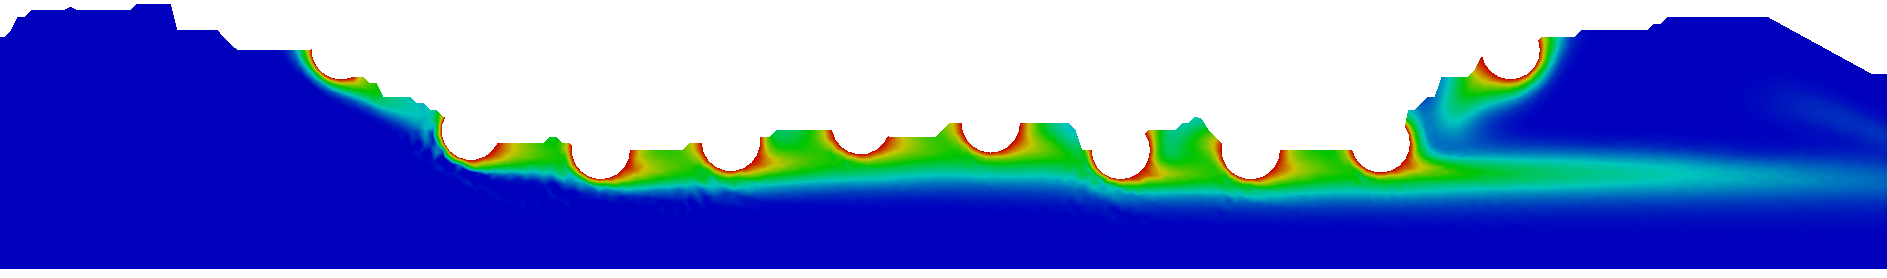
\includegraphics[scale=0.115]{./02_chaps/cap_solution/figure/conc10_RealStrut25000.png}\\
      t = 5.0
     \end{minipage}
     \begin{minipage}{.50\linewidth}
     \medskip
      \centering
      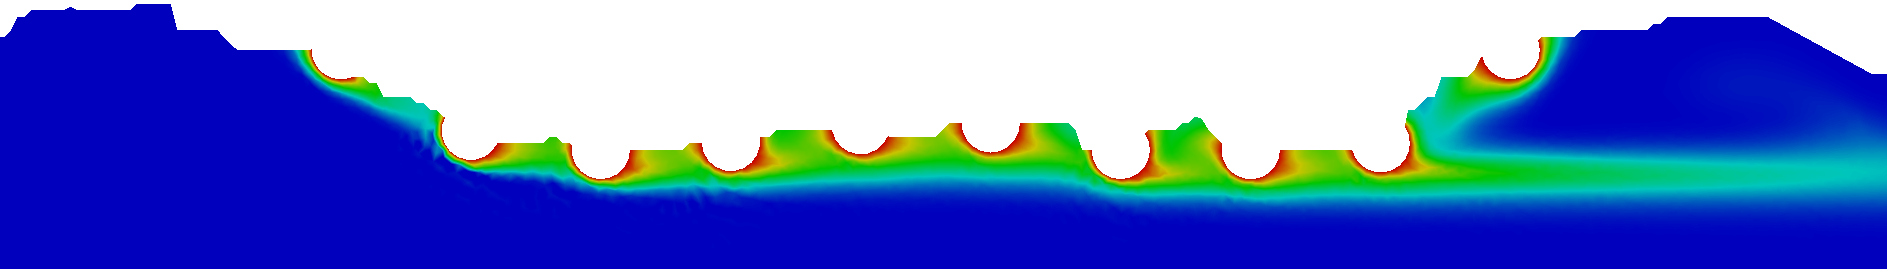
\includegraphics[scale=0.115]{./02_chaps/cap_solution/figure/conc10_RealStrut35000.png}\\
      t = 7.0
     \end{minipage}%
     \begin{minipage}{.50\linewidth}
     \medskip
      \centering
      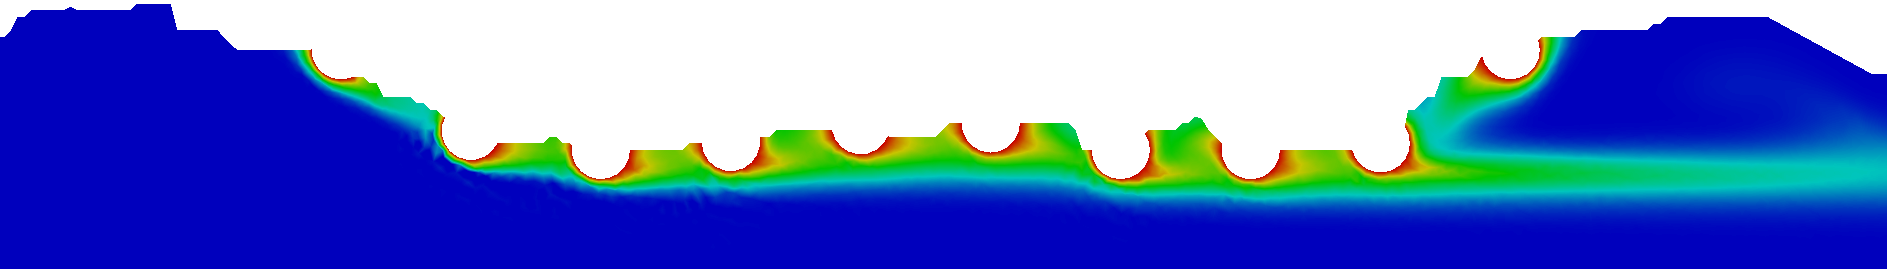
\includegraphics[scale=0.115]{./02_chaps/cap_solution/figure/conc10_RealStrut50000.png}\\
      t = 10.0
     \end{minipage}
     \medskip
     \caption{
ime and space evolution of the concentration field for real channel 
with drug-eluting stent when the $Sc=10$.}
     \label{conc field real stent sc 10}
\end{figure}


\newpage


